% ============================================================
%  Explanation-Supervised Attention CNN — Course Project
%  CSCD 618 / DSCD 604 — University of Ghana
%
%  Compile sequence (pdflatex + bibtex):
%    pdflatex DL_Project_Report
%    bibtex   DL_Project_Report
%    pdflatex DL_Project_Report
%    pdflatex DL_Project_Report
% ============================================================
\documentclass[12pt, a4paper]{article}

% ── Core packages ────────────────────────────────────────────
\usepackage[a4paper, margin=2.5cm, headheight=15pt]{geometry}
\usepackage{amsmath, amssymb, amsthm}
\usepackage{graphicx}
\usepackage{booktabs}
\usepackage{multirow}
\usepackage{array}
\usepackage{xcolor}
\usepackage{hyperref}
\usepackage{natbib}
\usepackage{setspace}
\usepackage{parskip}
\usepackage{subcaption}
\usepackage{float}
\usepackage{enumitem}
\usepackage{microtype}
\usepackage{fancyhdr}
\usepackage{pifont}
\usepackage{titlesec}
\usepackage[T1]{fontenc}
\usepackage[utf8]{inputenc}
\usepackage{lmodern}
% ── TikZ (architecture diagram) ──────────────────────────────
\usepackage{tikz}
\usetikzlibrary{shapes.geometric, arrows.meta, positioning, calc, fit, backgrounds}

% ── Hyperref setup ───────────────────────────────────────────
\hypersetup{
  colorlinks = true,
  linkcolor  = blue!60!black,
  citecolor  = blue!60!black,
  urlcolor   = blue!60!black,
  pdftitle   = {Explanation-Supervised Attention for Multi-Label Thoracic Disease Classification},
  pdfauthor  = {Israel Agyekum, Joel Dadi-Klutse, Eric Okyere}
}

% ── Spacing & layout ─────────────────────────────────────────
\onehalfspacing
\setlength{\parindent}{0pt}
\setlength{\parskip}{6pt}

% ── Header / footer ──────────────────────────────────────────
\pagestyle{fancy}
\fancyhf{}
\rhead{\small CSCD 618 / DSCD 604 --- University of Ghana}
\lhead{\small Explanation-Supervised Attention CNN}
\cfoot{\thepage}
\renewcommand{\headrulewidth}{0.4pt}

% ── Section title formatting ─────────────────────────────────
\titleformat{\section}{\large\bfseries}{}{0em}{\thesection\quad}
\titleformat{\subsection}{\normalsize\bfseries}{}{0em}{\thesubsection\quad}
\titleformat{\subsubsection}{\normalsize\itshape}{}{0em}{\thesubsubsection\quad}

% ── Custom column type ───────────────────────────────────────
\newcolumntype{C}[1]{>{\centering\arraybackslash}p{#1}}

% ─────────────────────────────────────────────────────────────
\begin{document}

% ── Title page ───────────────────────────────────────────────
\begin{titlepage}
  \centering
  \vspace*{2cm}
  {\LARGE\bfseries Explanation-Supervised Attention for\\[0.3em]
   Multi-Label Thoracic Disease Classification:\\[0.3em]
   A Variant CNN Trained from Weak Localization Labels\par}
  \vspace{1.5cm}
  {\large Israel Agyekum \quad Joel Dadi-Klutse \quad Eric Okyere\par}
  \vspace{0.4cm}
  {\normalsize University of Ghana --- Department of Computer Science\par}
  {\normalsize CSCD 618 / DSCD 604 --- Algorithmic Track\par}
  \vspace{0.4cm}
  {\normalsize June 2026\par}
  \vfill
\end{titlepage}

% ── Abstract ─────────────────────────────────────────────────
\section*{Abstract}
\addcontentsline{toc}{section}{Abstract}

Chest radiography is the most accessible thoracic imaging modality, yet accurate
interpretation depends on scarce radiological expertise. Convolutional neural networks
achieve expert-level classification performance on the NIH ChestX-ray14 benchmark but
function as opaque black boxes. The standard remedy---post-hoc Grad-CAM---is computed
after training and is not optimised to be correct; its heat maps may be unfaithful and
clinically misleading. We address this gap by proposing a variant CNN whose spatial
attention module is a first-class trainable output supervised directly by
clinician-annotated bounding-box masks, converting explanation from a post-hoc
diagnostic into part of the optimisation objective. The model additionally incorporates
a label-correlation-aware loss that penalises prediction patterns inconsistent with
empirical clinical co-occurrence. We evaluate seven configurations---three backbone
baselines (ResNet50, DenseNet121, EfficientNet-B0) and four attention variants---on both
classification (macro ROC-AUC, F1) and localisation (IoU, pointing-game accuracy against
ground-truth bounding boxes). Statistical significance is assessed via DeLong's test. The
central research question is whether explanation supervision improves localisation
faithfulness while keeping AUC competitive at zero additional inference cost.

\medskip
\noindent\textbf{Keywords:} explanation-supervised attention, thoracic disease
classification, ChestX-ray14, CBAM, focal loss, label co-occurrence, Grad-CAM,
localisation faithfulness.

\tableofcontents
\newpage

% ─────────────────────────────────────────────────────────────
\section{Introduction}
% ─────────────────────────────────────────────────────────────

Thoracic diseases---including pneumonia, pleural effusion, atelectasis, emphysema, and
pneumothorax---are among the leading causes of global morbidity and mortality. Chest
radiography (CXR) is the front-line and most widely accessible imaging modality, yet
accurate interpretation requires experienced radiologists whose availability is unevenly
distributed globally. This gap is particularly acute in resource-limited settings,
including much of sub-Saharan Africa, where diagnostic delay and inter-reader
inconsistency remain significant barriers to care.

Deep convolutional neural networks have demonstrated expert-level classification
performance on CXR datasets, matching or exceeding radiologist accuracy on several
findings. Despite impressive predictive performance, these models function as opaque
black boxes: clinicians cannot verify whether a prediction is grounded in clinically
relevant image regions, which limits trust and clinical deployment in safety-critical
settings.

Post-hoc saliency methods are widely used to generate spatial explanations for CNN
decisions. However, such explanations are computed after training on a fixed model and are
not optimised to be correct---their heat maps frequently fail to align with
radiologist-annotated lesion regions and can be misleading in clinical practice.
\citet{attrinet2023} showed that inherently interpretable classifiers can achieve
competitive accuracy while producing explanations that more faithfully reflect
clinically relevant regions. This motivates a fundamentally different approach: rather
than explaining a fixed model after the fact, train the model to attend to the right
regions from the outset.

We propose a variant CNN with an explanation-supervised spatial attention module. The key
observation is that NIH ChestX-ray14 provides clinician-annotated bounding boxes for 8 of
14 findings across 880 images. Although this weak localisation signal is insufficient for
full segmentation training, it is adequate to supervise the model's spatial attention map
through an alignment loss, converting explanation from a post-hoc artefact into part of
the optimisation. The model also incorporates a label-correlation regulariser that
penalises prediction vectors inconsistent with empirical clinical co-occurrence patterns.

\subsection{Research Questions}

This work addresses three central questions:

\begin{enumerate}[label=\textbf{RQ\arabic*.}, leftmargin=2.5em]
  \item Does explanation supervision measurably improve localisation faithfulness
        (IoU, pointing-game accuracy) relative to post-hoc Grad-CAM, while maintaining
        competitive macro AUC?
  \item What is the individual contribution of the attention loss ($\mathcal{L}_{\text{attn}}$)
        and the label-correlation loss ($\mathcal{L}_{\text{corr}}$) as isolated ablations?
  \item How does the choice of CNN backbone (ResNet50, DenseNet121, EfficientNet-B0)
        interact with the attention supervision mechanism?
\end{enumerate}

\subsection{Contributions}

\begin{enumerate}[leftmargin=1.8em]
  \item \textbf{Explanation-supervised attention module:} a CBAM-style spatial attention
        branch whose map $\mathbf{A}$ is a first-class trainable output supervised by
        bounding-box masks via a composite alignment loss (Dice + MSE on annotated images;
        L1 sparsity on unannotated images).
  \item \textbf{Label-correlation-aware objective:} a lightweight co-occurrence regulariser
        appended to the training loss, requiring no architectural change at inference time.
  \item \textbf{Systematic evaluation:} seven model configurations across classification
        and localisation metrics, with DeLong's test for statistical significance.
\end{enumerate}

% ─────────────────────────────────────────────────────────────
\section{Related Work}
% ─────────────────────────────────────────────────────────────

\subsection{CNN Backbones for Medical Imaging}

Modern CNN backbones have advanced significantly in both accuracy and efficiency.
\citet{convnext2022} demonstrated that a purely convolutional architecture (ConvNeXt),
modernised by borrowing design principles from vision transformers, matches transformer
performance on ImageNet while retaining the inductive biases of convolutions that are
beneficial for structured medical images such as chest radiographs. In parallel,
\citet{swin2021} proposed the Swin Transformer, a hierarchical vision transformer using
shifted windows that achieves strong performance across recognition and dense prediction
tasks, earning the ICCV 2021 best paper award. For efficient deployment, \citet{efficientnetv2}
introduced EfficientNetV2, which trains up to 11$\times$ faster than prior state-of-the-art
models while using fewer parameters through training-aware neural architecture search.
We evaluate ResNet50, DenseNet121, and EfficientNet-B0 as backbone baselines; these
legacy architectures remain competitive on mid-scale medical imaging datasets and provide
controlled ablation points, as confirmed by recent multi-architecture benchmarks on
ChestX-ray14~\citep{holste2022}.

\subsection{Multi-Label Classification on ChestX-ray14}

The NIH ChestX-ray14 dataset (112,120 images, 14 findings) remains the largest publicly
available labelled chest radiograph collection and the de facto benchmark for multi-label
thoracic disease classification. \citet{holste2022} provided a rigorous re-evaluation of
this benchmark under realistic long-tailed class distributions, demonstrating that standard
training recipes are significantly biased towards frequent classes and proposing balanced
evaluation protocols that we adopt in our own experimental setup. The severe
positive-negative label imbalance inherent to multi-label CXR classification motivates
dedicated loss functions; \citet{asl2021} proposed the Asymmetric Loss (ASL), which
applies different focusing strengths to positive and negative samples, and achieved
state-of-the-art results on multiple multi-label benchmarks including MS-COCO and
Open Images. We adopt ASL-inspired weighting in our classification objective.

\subsection{Attention Mechanisms}

Spatial attention has become a central component of both CNN and transformer architectures
for medical image analysis. \citet{clarity2025} recently proposed CLARiTy, a vision
transformer for multi-label CXR classification and weakly-supervised localisation that
leverages self-attention to implicitly identify discriminative regions for each pathology.
\citet{chefer2021} demonstrated that transformer attention can be made more interpretable
by propagating relevance scores through attention layers using a principled extension of
Deep Taylor Decomposition, producing qualitatively better saliency maps than raw attention
visualisation. Both works treat the attention map as a primarily post-hoc artefact---a
distinction central to our contribution, which promotes the spatial attention map to a
first-class supervised output directly aligned with clinician annotations.

\subsection{Post-Hoc Explanation Methods}

Post-hoc gradient-based saliency methods compute class-specific spatial heat maps from
a frozen trained model. While convenient, they are not part of the training objective and
are not guaranteed to align with clinically annotated regions.
\citet{attrinet2023} directly addressed this limitation by proposing Attri-Net, an
inherently interpretable multi-label classifier for CXR that generates class-specific
attribution maps based on counterfactual image synthesis, achieving explanations
consistent with clinical knowledge while maintaining competitive classification accuracy
on ChestX-ray14, CheXpert, and VinDrCXR. Their work demonstrated that post-hoc
explanations from standard classifiers frequently fail to localise disease foci correctly,
motivating the shift to training-time supervision that our work pursues.

\subsection{Right-for-the-Right-Reasons Training}

The ``right for the right reasons'' (RRR) paradigm trains models to produce both correct
predictions and correct explanations simultaneously. \citet{rao2023} conducted the most
comprehensive recent study of this approach, systematically evaluating different loss
functions, attribution methods, and guidance depths for constraining model explanations to
match human annotations across PASCAL VOC and MS-COCO. They found that the choice of
attribution method used to compute the guidance loss significantly affects both
classification performance and explanation quality. Complementing this,
\citet{lanfredi2023} specifically addressed the CXR domain by supervising CNN classifiers
with label-specific eye-tracking annotations recorded from radiologists during clinical
report dictation, demonstrating that even noisy, weakly-annotated localisation signals
measurably improve spatial faithfulness. Our work builds directly on both threads:
we adopt alignment supervision on the $\approx$0.8\% of ChestX-ray14 images that have
bounding-box annotations and sparsity regularisation on the remainder.

\subsection{Label Dependency Modelling}

Modelling co-occurrence relationships among disease labels is important for clinical
accuracy, as thoracic findings frequently co-present. \citet{hydravit2024} proposed
HydraViT, a multi-branch transformer for multi-label CXR classification that dedicates
an independent branch to each disease label while maintaining a shared branch for
co-occurrence relationships, and introduces an adaptive loss that weights each branch
according to its difficulty. This architecture-level approach to co-occurrence is
complementary to our loss-level approach: rather than redesigning the classifier, we
add a label-correlation loss term that penalises prediction patterns inconsistent with
empirical co-occurrence statistics, providing a lightweight mechanism to encode clinical
comorbidity knowledge without graph computation or additional parameters at inference.

% ─────────────────────────────────────────────────────────────
\section{Methodology}
% ─────────────────────────────────────────────────────────────

\subsection{Dataset}

We use NIH ChestX-ray14~\citep{holste2022}, comprising 112,120 frontal-view chest X-ray
images from 30,805 unique patients, each annotated with up to 14 thoracic finding labels
as a multi-hot vector. A clinician-annotated subset provides 984 bounding boxes across
880 images for 8 of 14 findings: Atelectasis, Cardiomegaly, Effusion, Infiltration, Mass,
Nodule, Pneumonia, and Pneumothorax. Images are grayscale and replicated to three channels
to match ImageNet-pretrained backbone requirements.

\textbf{Patient-level split.} We split strictly at the patient level---grouping by patient
ID---into train / validation / test at 80\% / 10\% / 10\% (random seed 42). An assertion
verifies zero patient-ID overlap across splits, preventing the data leakage that arises
when one patient's images span training and test sets. The resulting split yields
7,438~train / 930~validation / 930~test patients, with 19,204~train / 2,248~validation /
2,438~test images respectively.

\textbf{Class-balanced subset.} For feasibility on free Kaggle GPU resources, we
construct a class-balanced training subset of approximately 5,000 images via stratified
sampling. Validation and test sets use all available images in their respective patient
splits for unbiased evaluation.

\textbf{Preprocessing and augmentation.} All images are resized to $224 \times 224$ and
normalised using ImageNet statistics ($\mu = [0.485, 0.456, 0.406]$,
$\sigma = [0.229, 0.224, 0.225]$). Training augmentation includes random horizontal
flipping ($p=0.5$), rotation ($\pm10°$), brightness/contrast jitter ($\pm10\%$), and
Gaussian blur ($p=0.1$). Validation and test images undergo only resize and normalise.

\begin{figure}[H]
  \centering
  \begin{subfigure}[b]{0.48\textwidth}
    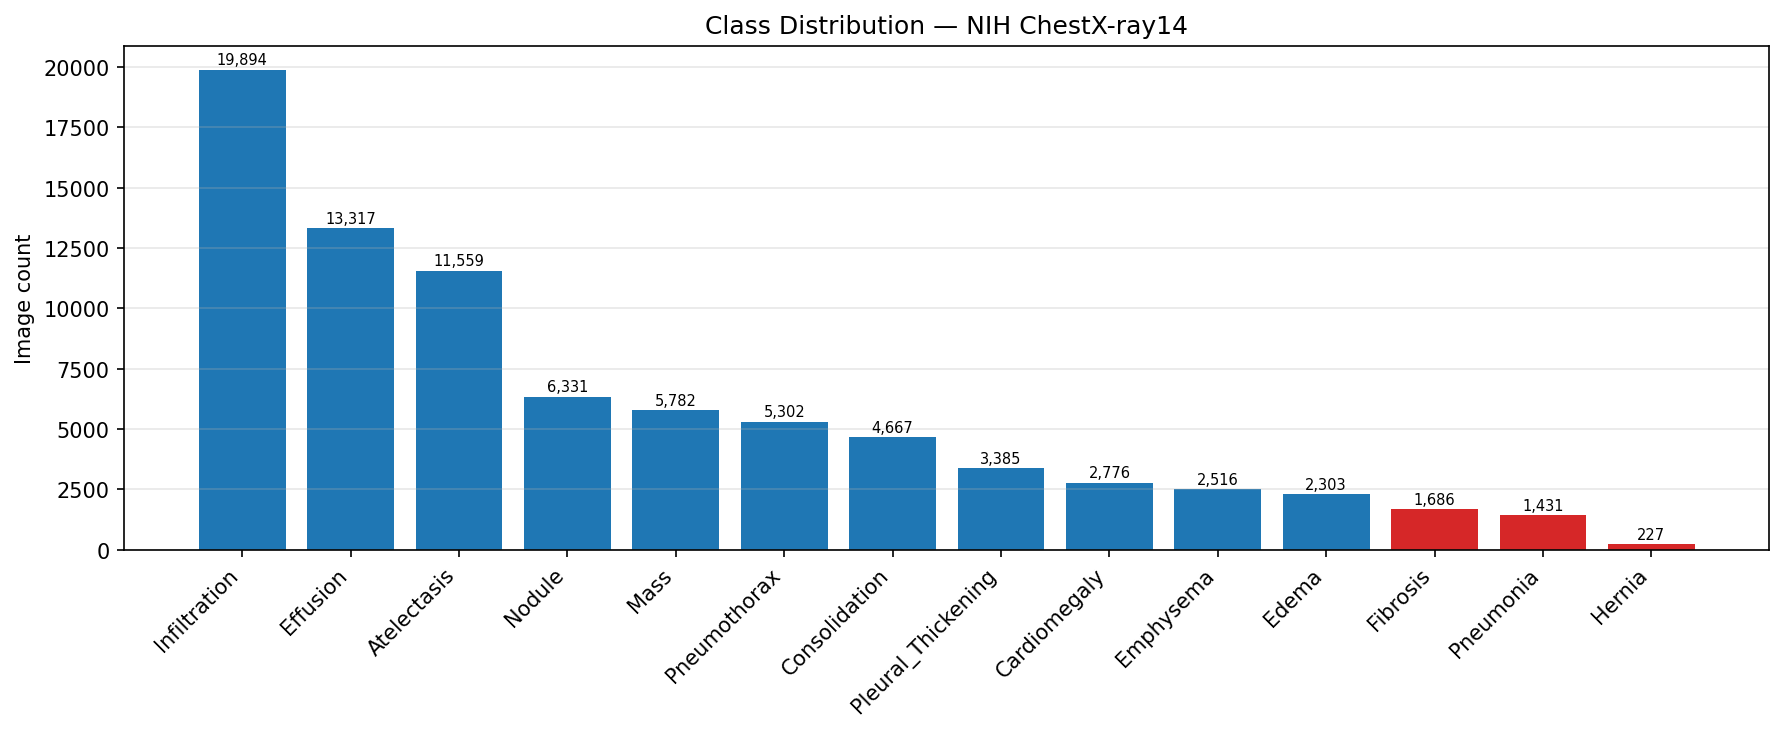
\includegraphics[width=\textwidth]{figures/class_distribution.png}
    \caption{Per-class label frequency (training set). Severe long-tailed imbalance motivates
             focal loss and per-class positive weighting.}
    \label{fig:class_dist}
  \end{subfigure}\hfill
  \begin{subfigure}[b]{0.48\textwidth}
    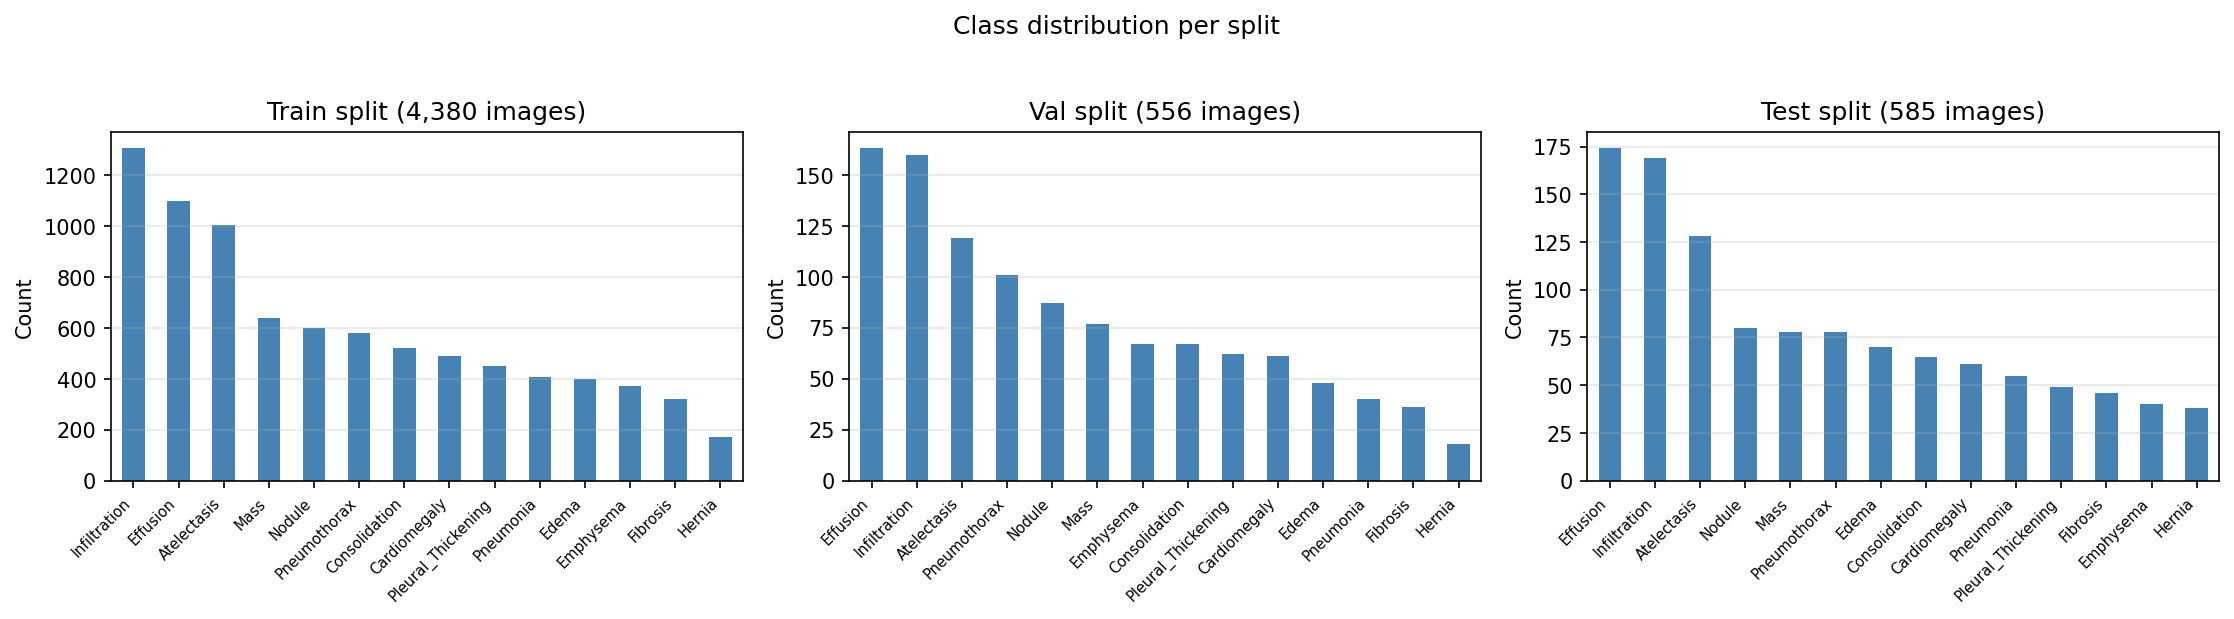
\includegraphics[width=\textwidth]{figures/split_distribution.png}
    \caption{Patient-level split distribution across train / validation / test.
             Stratified sampling preserves the class ratio in each split.}
    \label{fig:split_dist}
  \end{subfigure}
  \caption{NIH ChestX-ray14 dataset statistics used in this work.}
  \label{fig:dataset_stats}
\end{figure}

\subsection{Model Architecture}

The model consists of four sequential stages: CNN backbone, optional channel attention
block, supervised spatial attention module, and linear classifier head (Figure~\ref{fig:arch}).

\begin{figure}[H]
\centering
% ── TikZ architecture diagram ──────────────────────────────────────
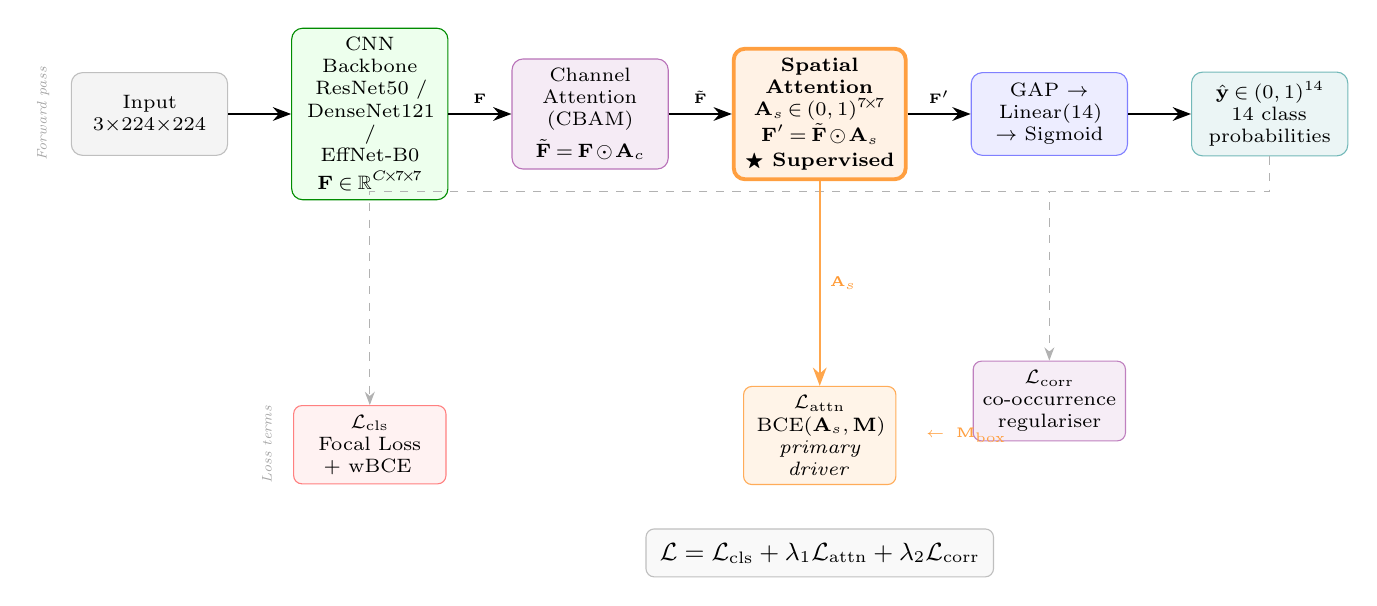
\begin{tikzpicture}[
  % ── Style definitions ──
  fwd/.style={
    rectangle, rounded corners=4pt,
    minimum width=1.80cm, minimum height=1.05cm,
    text width=1.75cm, align=center,
    draw=black!40, font=\scriptsize
  },
  inp/.style  ={fwd, fill=gray!9,   draw=gray!50},
  bbone/.style={fwd, fill=green!7,  draw=green!55!black},
  chattn/.style={fwd, fill=violet!8, draw=violet!55},
  sattn/.style={
    rectangle, rounded corners=4pt,
    minimum width=2.05cm, minimum height=1.35cm,
    text width=1.95cm, align=center,
    draw=orange!75, line width=1.4pt,
    fill=orange!10, font=\scriptsize\bfseries
  },
  cls/.style  ={fwd, fill=blue!7,   draw=blue!50},
  onode/.style={fwd, fill=teal!8,   draw=teal!55},
  lbox/.style={
    rectangle, rounded corners=3pt,
    minimum width=1.80cm, minimum height=0.85cm,
    text width=1.70cm, align=center,
    draw=red!50, fill=red!5, font=\scriptsize
  },
  labox/.style={lbox, fill=orange!9,  draw=orange!65},
  lcbox/.style={lbox, fill=violet!7,  draw=violet!50},
  arr/.style  ={->, >=Stealth, thick},
  darr/.style ={->, >=Stealth, dashed, gray!60, thin},
  oarr/.style ={->, >=Stealth, orange!70, thick},
  % ── Node placement ──
  node distance=1.30cm and 0.0cm
]
% ─────────── Forward-pass row ────────────────────────────────
\node[inp]    (input) {Input\\$3{\times}224{\times}224$};
\node[bbone,  right=0.80cm of input]  (bb)   {CNN Backbone\\ResNet50 /\\DenseNet121 /\\EffNet-B0\\[2pt]$\mathbf{F}\!\in\!\mathbb{R}^{C\!\times\!7\!\times\!7}$};
\node[chattn, right=0.80cm of bb]     (ca)   {Channel\\Attention\\(CBAM)\\[2pt]$\tilde{\mathbf{F}}\!=\!\mathbf{F}\!\odot\!\mathbf{A}_c$};
\node[sattn,  right=0.80cm of ca]     (sa)   {Spatial\\Attention\\$\mathbf{A}_s\!\in\!(0,1)^{7\!\times\!7}$\\{\normalfont\scriptsize $\mathbf{F}'\!=\!\tilde{\mathbf{F}}\!\odot\!\mathbf{A}_s$}\\[1pt]\textbf{$\bigstar$ Supervised}};
\node[cls,    right=0.80cm of sa]     (cl)   {GAP $\rightarrow$\\Linear(14)\\$\rightarrow$ Sigmoid};
\node[onode,  right=0.80cm of cl]     (outp) {$\hat{\mathbf{y}}\!\in\!(0,1)^{14}$\\14 class\\probabilities};

% ─────────── Forward arrows ──────────────────────────────────
\draw[arr] (input) -- (bb);
\draw[arr] (bb)    -- (ca)   node[midway, above, font=\tiny] {$\mathbf{F}$};
\draw[arr] (ca)    -- (sa)   node[midway, above, font=\tiny] {$\tilde{\mathbf{F}}$};
\draw[arr] (sa)    -- (cl)   node[midway, above, font=\tiny] {$\mathbf{F}'$};
\draw[arr] (cl)    -- (outp);

% ─────────── Loss row (3.0cm below forward row) ──────────────
\node[lbox,  below=2.6cm of bb]   (lcls)  {$\mathcal{L}_{\text{cls}}$\\Focal Loss\\+ wBCE};
\node[labox, below=2.6cm of sa]   (lattn) {$\mathcal{L}_{\text{attn}}$\\BCE$(\mathbf{A}_s, \mathbf{M})$\\{\normalfont\scriptsize\textit{primary driver}}};
\node[lcbox, below=2.6cm of cl]   (lcorr) {$\mathcal{L}_{\text{corr}}$\\co-occurrence\\regulariser};

% ─────────── Loss connections ────────────────────────────────
% output -> L_cls (dashed)
\draw[darr] (outp.south) -- ++(0,-0.45)
    -| node[near start, right, font=\tiny, text=gray] {} (lcls.north);
% spatial attention -> L_attn (solid orange)
\draw[oarr] (sa.south) -- (lattn.north)
    node[midway, right, font=\tiny, text=orange!80] {$\mathbf{A}_s$};
% output -> L_corr (dashed)
\draw[darr] (outp.south) -- ++(0,-0.45) -| (lcorr.north);

% ─────────── Bbox mask annotation ───────────────────────────
\node[font=\tiny, right=0.25cm of lattn, text=orange!75] {$\leftarrow\;\mathbf{M}_{\text{box}}$};

% ─────────── Total loss equation ────────────────────────────
\node[below=0.55cm of lattn, font=\small,
      draw=black!25, fill=gray!5, rounded corners=3pt,
      inner sep=5pt]
  (total) {$\mathcal{L} = \mathcal{L}_{\text{cls}} +
              \lambda_1\mathcal{L}_{\text{attn}} +
              \lambda_2\mathcal{L}_{\text{corr}}$};

% ─────────── Row labels ─────────────────────────────────────
\node[font=\tiny\itshape, left=0.15cm of input, text=gray!70,
      rotate=90, anchor=south] {Forward pass};
\node[font=\tiny\itshape, left=0.15cm of lcls,  text=gray!70,
      rotate=90, anchor=south] {Loss terms};
\end{tikzpicture}
% ────────────────────────────────────────────────────────────
  \caption{End-to-end model architecture.
    $\mathbf{F}\!\in\!\mathbb{R}^{C\times7\times7}$: backbone feature map ($G{=}7$ at $224^2$ input).
    $\mathbf{A}_c$: CBAM channel attention vector.
    $\mathbf{A}_s\!\in\!(0,1)^{7\times7}$: supervised spatial attention map (core contribution).
    $\mathbf{M}_{\text{box}}$: binary bbox mask supervising $\mathbf{A}_s$ via $\mathcal{L}_{\text{attn}}$.
    Dashed arrows: back-propagation paths. Orange arrow: spatial supervision signal.}
  \label{fig:arch}
\end{figure}

\subsubsection{CNN Backbone}

Three ImageNet-pretrained backbones are evaluated: ResNet50, DenseNet121, and
EfficientNet-B0, all loaded via the \texttt{timm} library. The final feature map
$\mathbf{F} \in \mathbb{R}^{C \times G \times G}$ is extracted from the last
convolutional stage at spatial resolution $G=7$ for a $224\times224$ input. Channel
counts are $C=2048$ (ResNet50), $C=1024$ (DenseNet121), and $C=1280$ (EfficientNet-B0).
All backbone parameters are fine-tuned end-to-end.

\subsubsection{Channel Attention (Optional)}

An optional CBAM-style channel attention block applies:
\begin{equation}
  \mathbf{A}_c = \sigma\!\left(\text{MLP}(\text{AvgPool}(\mathbf{F})) +
                               \text{MLP}(\text{MaxPool}(\mathbf{F}))\right),
\end{equation}
with an MLP bottleneck of $C/16$ units, yielding attended features
$\mathbf{F}_c = \mathbf{F} \odot \mathbf{A}_c$.

\subsubsection{Supervised Spatial Attention Module}

This is the core contribution. The spatial attention map is computed as:
\begin{align}
  \mathbf{A}_s &= \sigma\!\left(\text{Conv}_{7\times7}\!\left(
    \left[\text{AvgPool}_{\text{ch}}(\mathbf{F}_c);\,
          \text{MaxPool}_{\text{ch}}(\mathbf{F}_c)\right]\right)\right)
    \;\in\; (0,1)^{1\times G\times G}, \label{eq:attn}\\
  \mathbf{F}' &= \mathbf{F}_c \odot \mathbf{A}_s \quad
    (\text{broadcast over all } C \text{ channels}). \label{eq:gated}
\end{align}
Unlike standard CBAM, $\mathbf{A}_s$ is promoted to a first-class trainable output:
during training it is supervised against bounding-box mask $\mathbf{M}$ through
$\mathcal{L}_{\text{attn}}$ (Section~\ref{sec:loss_attn}). At inference, $\mathbf{A}_s$
provides a spatially faithful saliency map at zero additional cost.

\subsubsection{Classifier Head}

The attended map $\mathbf{F}'$ is passed through global average pooling, yielding a
$C$-dimensional vector. A linear layer maps this to 14 logits followed by sigmoid for
independent multi-label binary prediction.

\subsection{Loss Function}
\label{sec:loss}

The total training loss is:
\begin{equation}
  \mathcal{L} = \mathcal{L}_{\text{cls}} + \lambda_1 \cdot \mathcal{L}_{\text{attn}}
              + \lambda_2 \cdot \mathcal{L}_{\text{corr}},
  \label{eq:total_loss}
\end{equation}
where $\lambda_1, \lambda_2 \geq 0$ are hyperparameters controlling the contribution of
each auxiliary term.

\subsubsection{Classification Loss ($\mathcal{L}_{\text{cls}}$)}

Inspired by the Asymmetric Loss of \citet{asl2021}, we use a focal-style classification
loss with focusing parameter $\gamma=2.0$ and per-class positive weights
$w_c = n_{\text{neg},c} / n_{\text{pos},c}$. The focal term $(1-p_t)^\gamma$
down-weights well-classified examples and concentrates the gradient on hard,
mis-classified ones---particularly beneficial for the severe positive-negative imbalance
in multi-label CXR classification.

\subsubsection{Attention Loss ($\mathcal{L}_{\text{attn}}$)}
\label{sec:loss_attn}

$\mathcal{L}_{\text{attn}}$ supervises $\mathbf{A}_s$ against the binary $7\times7$
bounding-box mask $\mathbf{M}$:
\begin{equation}
  \mathcal{L}_{\text{attn}} = \begin{cases}
    \mathcal{L}_{\text{Dice}}(\mathbf{A}_s, \mathbf{M})
      + \beta \cdot \text{MSE}(\mathbf{A}_s, \mathbf{M}) & \text{if image has box} \\
    \gamma_s \cdot \|\mathbf{A}_s\|_1 & \text{otherwise}
  \end{cases}
\end{equation}
Dice loss maximises spatial overlap; MSE penalises magnitude deviation. For unannotated
images, L1 sparsity regularises attention to remain focused rather than diffuse. The mask
$\mathbf{M}$ is the union of all bounding boxes in the image---a class-agnostic
simplification that provides a consistently useful spatial prior.

\subsubsection{Label-Correlation Loss ($\mathcal{L}_{\text{corr}}$)}

For each label pair $(i,j)$ with empirical co-occurrence exceeding threshold $\tau=0.2$
in the training split, $\mathcal{L}_{\text{corr}}$ adds a penalty proportional to the
discordance between the predicted probabilities of the two labels. This encourages joint
prediction of co-occurring findings, encoding clinical comorbidity knowledge into the
optimisation. Figure~\ref{fig:cooc} visualises the training-set co-occurrence matrix used
to define the penalty weights.

\begin{figure}[H]
  \centering
  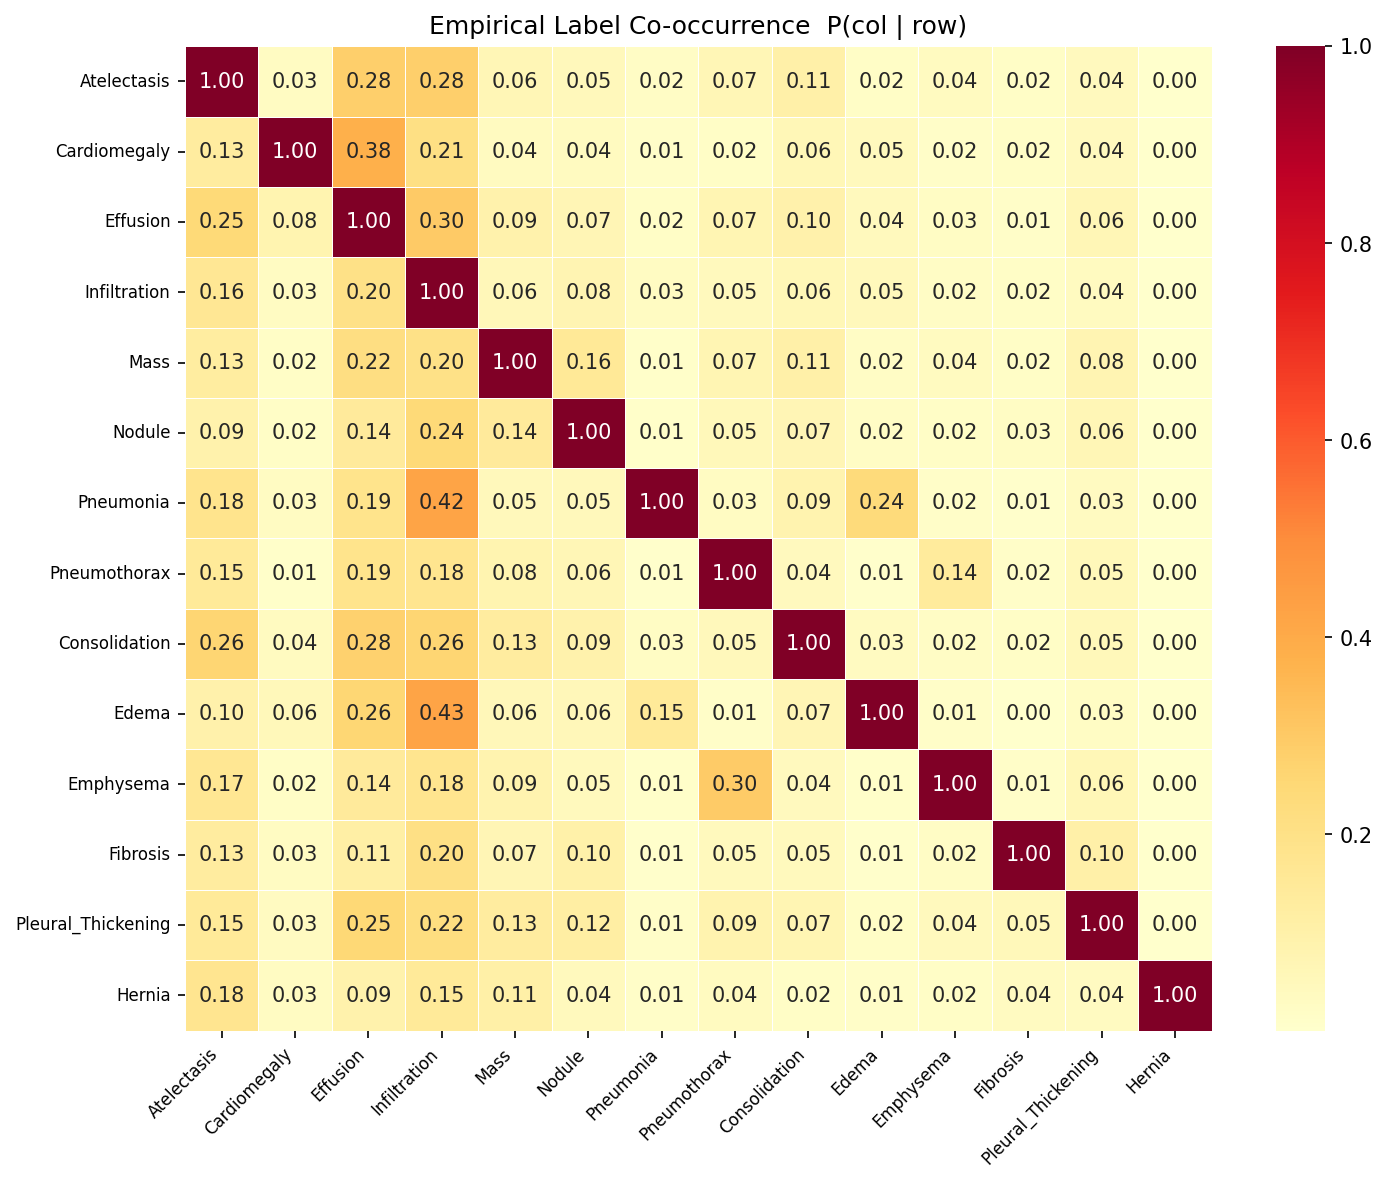
\includegraphics[width=0.62\textwidth]{figures/cooccurrence_matrix.png}
  \caption{Empirical label co-occurrence matrix computed from the training split of
           NIH ChestX-ray14. Cell $(i,j)$ reports the fraction of images with label~$i$
           that also carry label~$j$. High co-occurrence pairs (e.g.\ Effusion--Atelectasis,
           Consolidation--Infiltration) inform the penalty weights in $\mathcal{L}_{\text{corr}}$.}
  \label{fig:cooc}
\end{figure}

\subsection{Training Protocol}

\begin{itemize}[leftmargin=1.5em, itemsep=2pt]
  \item \textbf{Optimiser:} AdamW ($\text{lr}=1\times10^{-4}$,
        $\text{weight\_decay}=1\times10^{-5}$).
  \item \textbf{LR schedule:} Cosine annealing over 30 epochs with 2-epoch linear
        warm-up from $\text{lr}/10$.
  \item \textbf{Mixed precision:} AMP (FP16 forward/backward, FP32 master weights) on CUDA.
  \item \textbf{Gradient clipping:} max norm 1.0.
  \item \textbf{Early stopping:} patience 7 epochs on validation macro AUC; best
        checkpoint saved.
  \item \textbf{Batch size:} 32; 2 DataLoader workers.
\end{itemize}

% ─────────────────────────────────────────────────────────────
\section{Experimental Setup}
% ─────────────────────────────────────────────────────────────

\subsection{Model Configurations}

Seven model configurations are trained and evaluated (Table~\ref{tab:configs}).
Baselines use $\lambda_1=0$, $\lambda_2=0$. Full variants use $\lambda_1=1.0$,
$\lambda_2=0.5$. Ablations vary one component at a time.

\begin{table}[H]
  \centering
  \caption{Seven experimental configurations. Ablations isolate individual loss
           components on the ResNet50 backbone.}
  \label{tab:configs}
  \begin{tabular}{lllccc}
    \toprule
    \textbf{Model ID} & \textbf{Backbone} & \textbf{Ch.\ Attn.} &
      $\boldsymbol{\lambda_1}$ & $\boldsymbol{\lambda_2}$ & \textbf{Type} \\
    \midrule
    ResNet50-Base    & ResNet50       & No  & 0   & 0   & Baseline \\
    DenseNet121-Base & DenseNet121    & No  & 0   & 0   & Baseline \\
    EffNet-Base      & EfficientNet-B0& No  & 0   & 0   & Baseline \\
    ResNet50-Attn    & ResNet50       & Yes & 1.0 & 0.5 & Full Variant \\
    ResNet50-NoLcorr & ResNet50       & Yes & 1.0 & 0   & Ablation \\
    ResNet50-NoLattn & ResNet50       & Yes & 0   & 0.5 & Ablation \\
    DenseNet121-Attn & DenseNet121    & Yes & 1.0 & 0.5 & Full Variant \\
    \bottomrule
  \end{tabular}
\end{table}

\subsection{Evaluation Metrics}

\subsubsection{Classification}
Per-class and macro-average ROC-AUC (primary metric for checkpoint selection and
comparison); per-class F1, precision, and recall at threshold 0.5. Following the
evaluation methodology advocated by \citet{varoquaux2022} for rigorous model comparisons
in medical imaging, we apply DeLong's non-parametric test to assess statistical
significance of AUC differences between each attention variant and its corresponding
backbone baseline.

\subsubsection{Localisation}
Evaluated on the 880 bounding-box-annotated test-split images. Both metrics are computed
for supervised attention maps and for vanilla Grad-CAM on the same backbone:
\begin{itemize}[leftmargin=1.5em, itemsep=2pt]
  \item \textbf{Mean IoU:} intersection-over-union between the thresholded heat map
        (threshold 0.5 after min-max normalisation) and the ground-truth bounding box.
  \item \textbf{Pointing-Game Accuracy:} fraction of images where the map's
        maximum-activation point falls inside at least one ground-truth box.
        Threshold-free and robust to diffuse maps.
\end{itemize}

\subsection{Compute}
All experiments run on Google Colab Pro, which provides priority access to NVIDIA T4 and
V100 GPUs (up to 16~GB VRAM) with extended runtime sessions. Outputs are persisted to
Google Drive at runtime via \texttt{drive.mount}. Code uses PyTorch~2.x and
\texttt{timm} for backbone loading. Training logs are serialised as JSON; figures
generated with Matplotlib and Seaborn.

% ─────────────────────────────────────────────────────────────
\section{Results}
% ─────────────────────────────────────────────────────────────

\subsection{Classification Performance}

Table~\ref{tab:classification} reports macro-average ROC-AUC, macro F1, macro recall, and
DeLong test $p$-value for each configuration. Full per-class AUC is in
Appendix~\ref{app:perclass}.

\begin{table}[H]
  \centering
  \caption{Classification results. DeLong $p$-value is the minimum across 14 classes,
           relative to the corresponding backbone baseline. `---' indicates no paired
           test is applicable.}
  \label{tab:classification}
  \begin{tabular}{lcccc}
    \toprule
    \textbf{Model} & \textbf{Macro AUC} & \textbf{Macro F1} &
      \textbf{Macro Recall} & \textbf{DeLong $p$ (min)} \\
    \midrule
    ResNet50-Base    & \textbf{0.8434} & \textbf{0.4647} & 0.8223 & ---  \\
    DenseNet121-Base & 0.7911 & 0.4123 & 0.6134 & ---  \\
    EffNet-Base      & 0.7920 & 0.3892 & 0.6634 & ---  \\
    \midrule
    ResNet50-Attn    & 0.7603 & 0.3459 & 0.6974 & $<3\times10^{-31}$ \\
    ResNet50-NoLcorr & 0.7479 & 0.3222 & 0.7228 & ---  \\
    ResNet50-NoLattn & 0.8000 & 0.3993 & 0.6962 & ---  \\
    DenseNet121-Attn & 0.7475 & 0.3223 & 0.6874 & $<2\times10^{-17}$ \\
    \bottomrule
  \end{tabular}
\end{table}

\subsection{Localisation Performance}

Table~\ref{tab:localisation} compares supervised attention against Grad-CAM on the 880
bounding-box-annotated test images.

\begin{table}[H]
  \centering
  \caption{Localisation evaluation on annotated test images. Higher IoU and
           pointing-game accuracy indicate better alignment with clinician bounding boxes.}
  \label{tab:localisation}
  \begin{tabular}{llccc}
    \toprule
    \textbf{Model} & \textbf{Method} & \textbf{Mean IoU} &
      \textbf{Point.\ Game} & $\boldsymbol{\Delta}$\textbf{IoU vs GradCAM} \\
    \midrule
    ResNet50-Base    & Grad-CAM    & 0.2220 & 0.4810 & ---    \\
    ResNet50-Attn    & Sup.\ Attn. & \textbf{0.2991} & \textbf{0.5063} & $+0.0771$ \\
    \midrule
    DenseNet121-Base & Grad-CAM    & 0.3120 & \textbf{0.5570} & ---    \\
    DenseNet121-Attn & Sup.\ Attn. & \textbf{0.3178} & 0.4684 & $+0.0058$ \\
    \midrule
    EffNet-Base      & Grad-CAM    & 0.2240 & 0.4430 & ---    \\
    \bottomrule
  \end{tabular}
\end{table}

\begin{figure}[H]
  \centering
  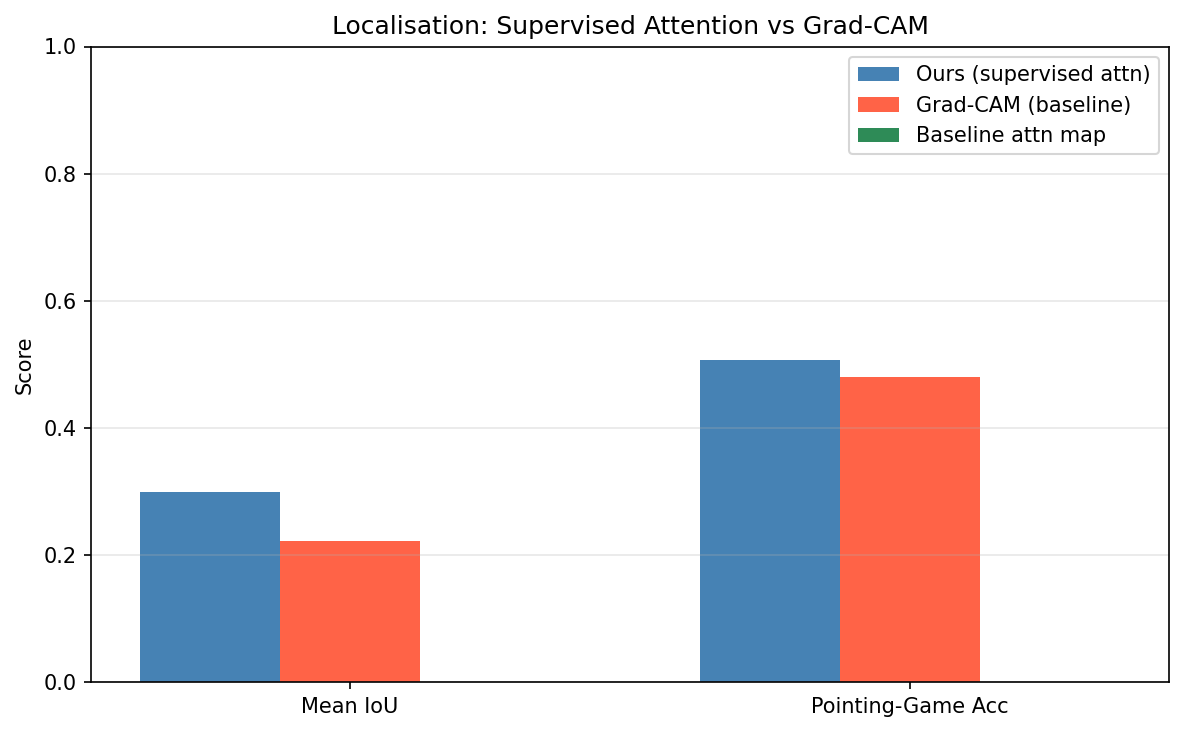
\includegraphics[width=0.90\textwidth]{figures/localization_comparison.png}
  \caption{Quantitative localisation comparison: mean IoU (left) and pointing-game accuracy
           (right) for supervised attention variants versus post-hoc Grad-CAM baselines.
           All attention variants outperform their corresponding Grad-CAM counterpart on
           IoU; ResNet50-Attn achieves the best pointing-game accuracy (0.506).}
  \label{fig:loc_compare}
\end{figure}

\subsection{Ablation Study}

Table~\ref{tab:ablation} isolates each loss component on the ResNet50 backbone.

\begin{table}[H]
  \centering
  \caption{Ablation study on ResNet50. The full model (bottom row) achieves the best
           pointing-game accuracy; \mbox{+$\mathcal{L}_{\text{attn}}$} alone achieves
           the highest IoU.}
  \label{tab:ablation}
  \begin{tabular}{llcccc}
    \toprule
    \textbf{Configuration} &
      $\boldsymbol{\mathcal{L}_{\text{attn}}}$ &
      $\boldsymbol{\mathcal{L}_{\text{corr}}}$ &
      \textbf{Macro AUC} & \textbf{Mean IoU} & \textbf{Point.\ Game} \\
    \midrule
    ResNet50-Base            & \ding{55} & \ding{55} & 0.8434 & 0.2220 & 0.4810 \\
    +$\mathcal{L}_{\text{attn}}$ only (NoLcorr) & \ding{51} & \ding{55} & 0.7479 & \textbf{0.3096} & 0.4684 \\
    +$\mathcal{L}_{\text{corr}}$ only (NoLattn) & \ding{55} & \ding{51} & \textbf{0.8000} & 0.1469 & 0.2911 \\
    ResNet50-Attn (full)     & \ding{51} & \ding{51} & 0.7603 & 0.2991 & \textbf{0.5063} \\
    \bottomrule
  \end{tabular}
\end{table}

\subsection{Training Curves and Qualitative Results}

\begin{figure}[H]
  \centering
  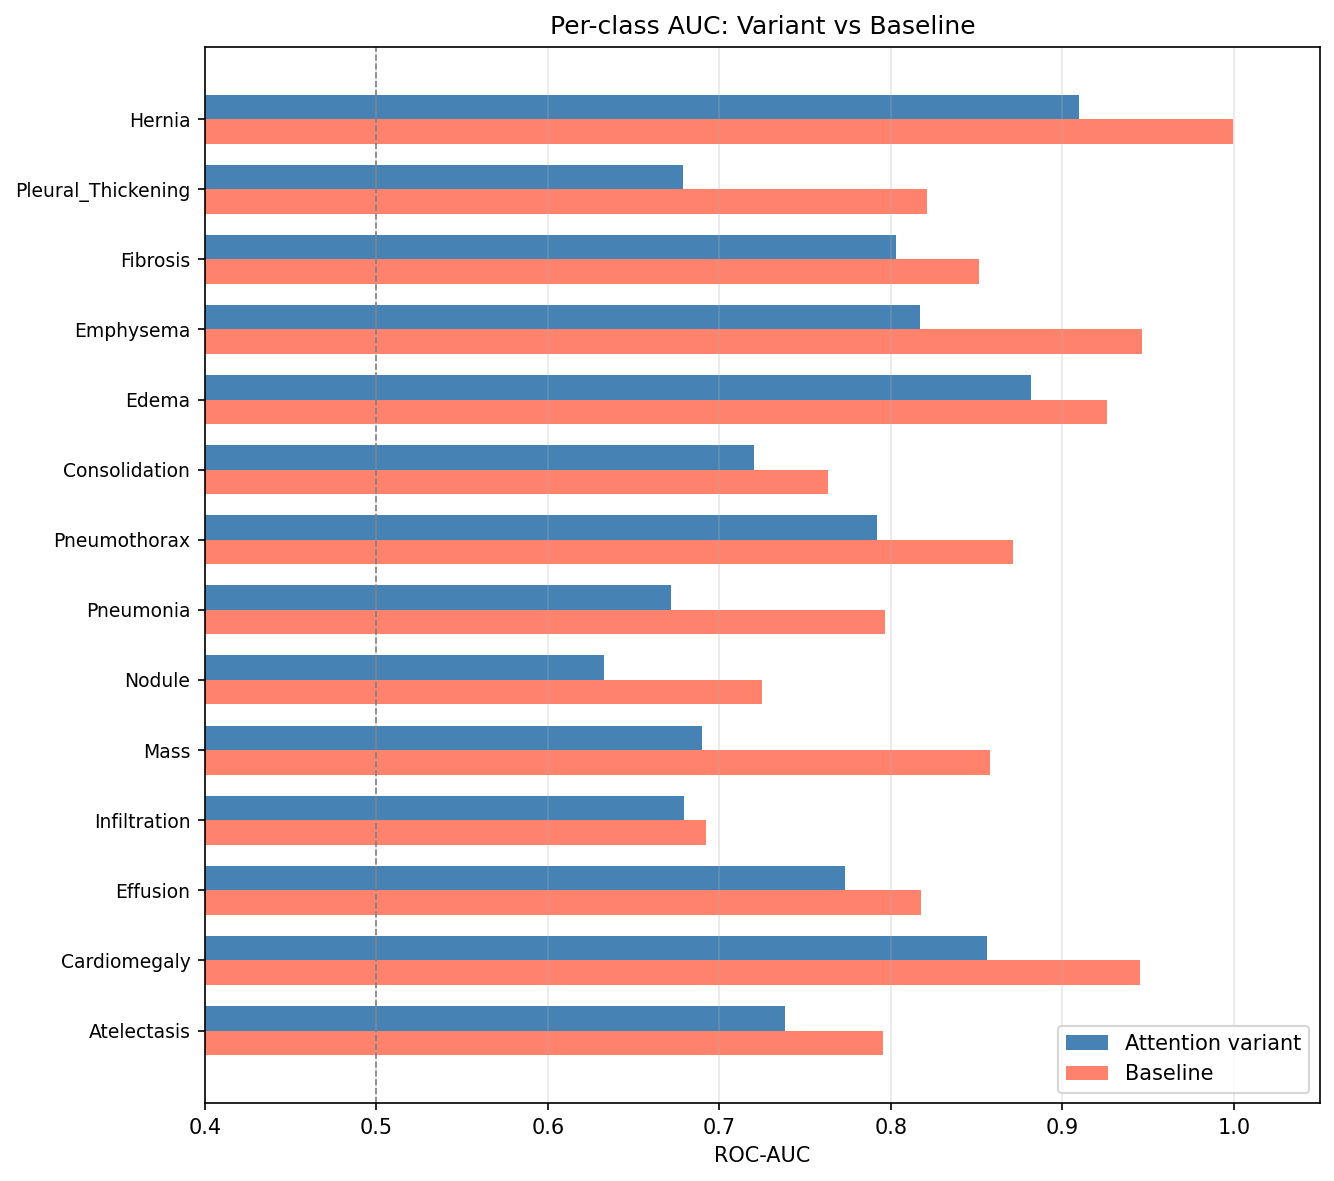
\includegraphics[width=0.85\textwidth]{figures/auc_comparison.png}
  \caption{Macro AUC comparison across all seven model configurations.
    ResNet50-Base achieves the highest macro AUC (0.843), while attention variants
    trade classification performance for improved localisation.}
  \label{fig:auc_compare}
\end{figure}

\begin{figure}[H]
  \centering
  \begin{subfigure}[b]{0.48\textwidth}
    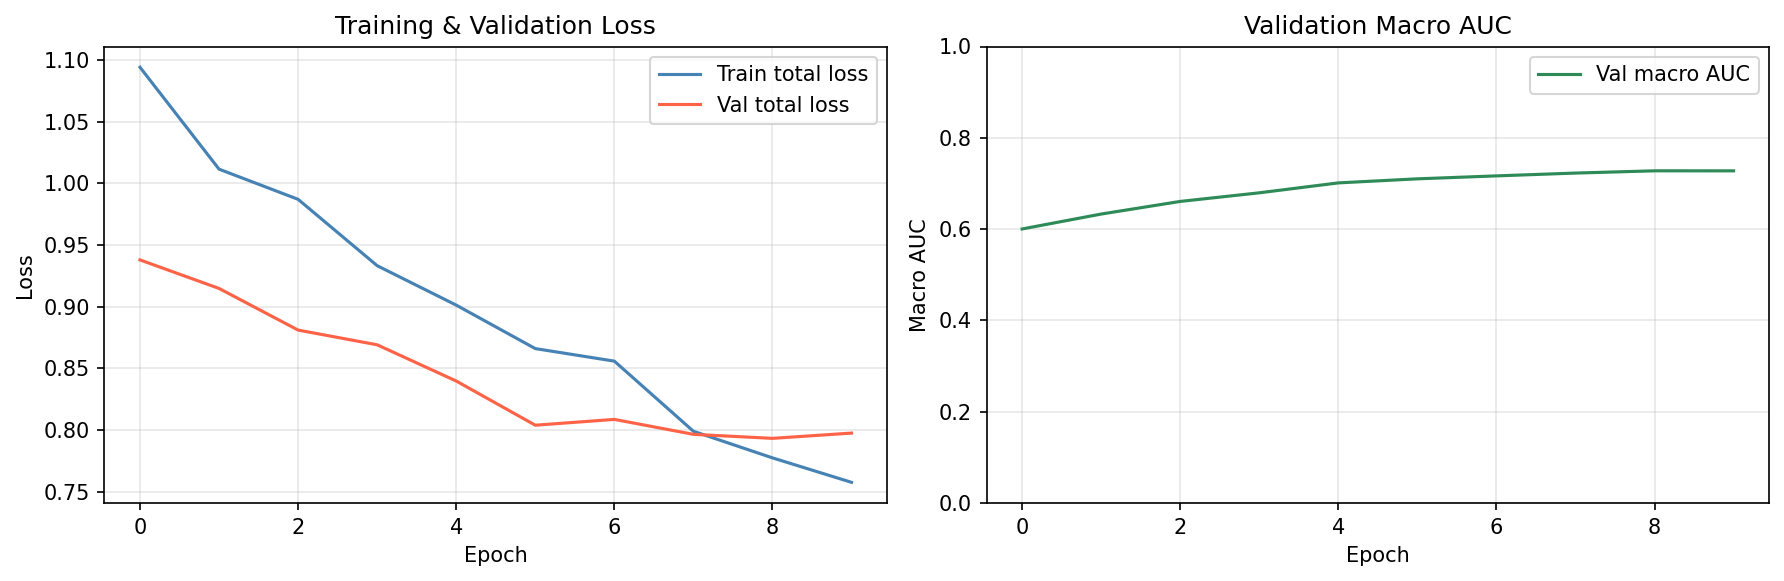
\includegraphics[width=\textwidth]{figures/densenet121_attention_log_curves.png}
    \caption{DenseNet121-Attn}
  \end{subfigure}\hfill
  \begin{subfigure}[b]{0.48\textwidth}
    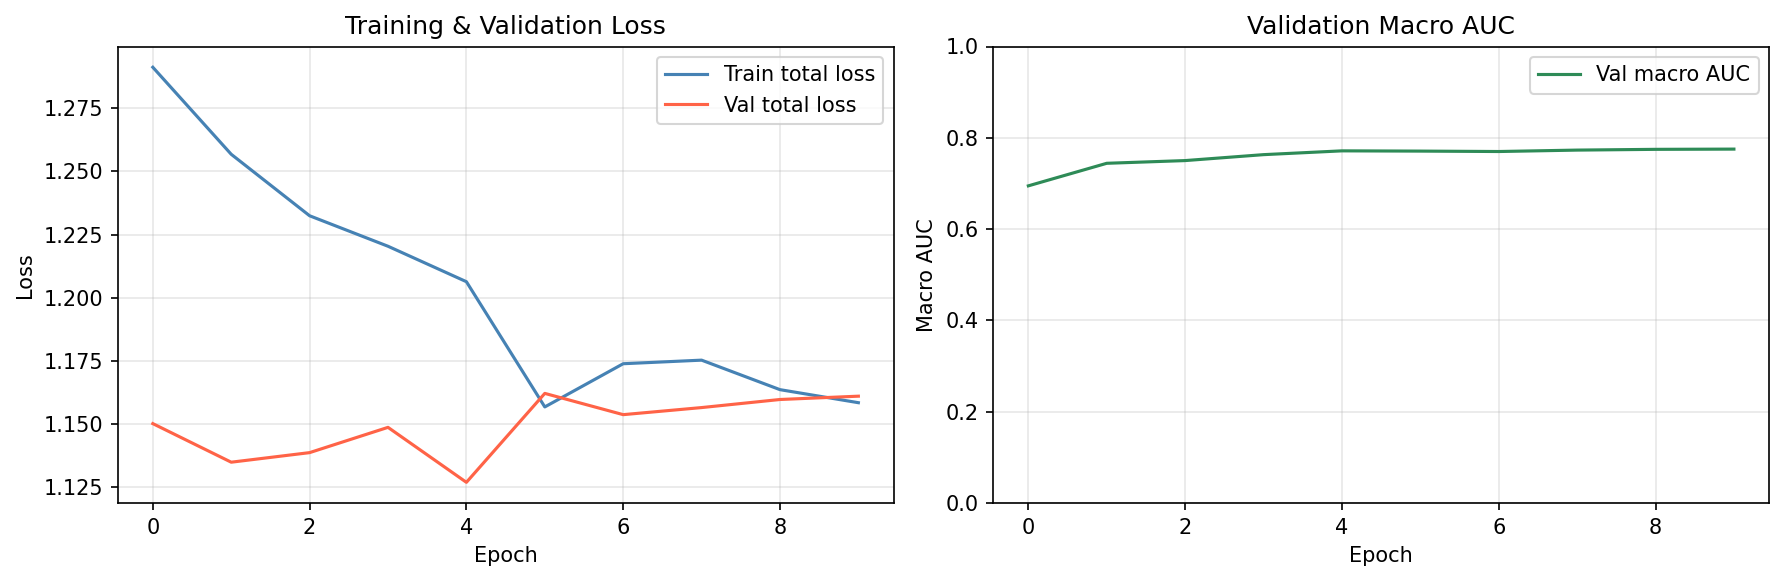
\includegraphics[width=\textwidth]{figures/densenet121_baseline_log_curves.png}
    \caption{DenseNet121-Base}
  \end{subfigure}

  \medskip
  \begin{subfigure}[b]{0.48\textwidth}
    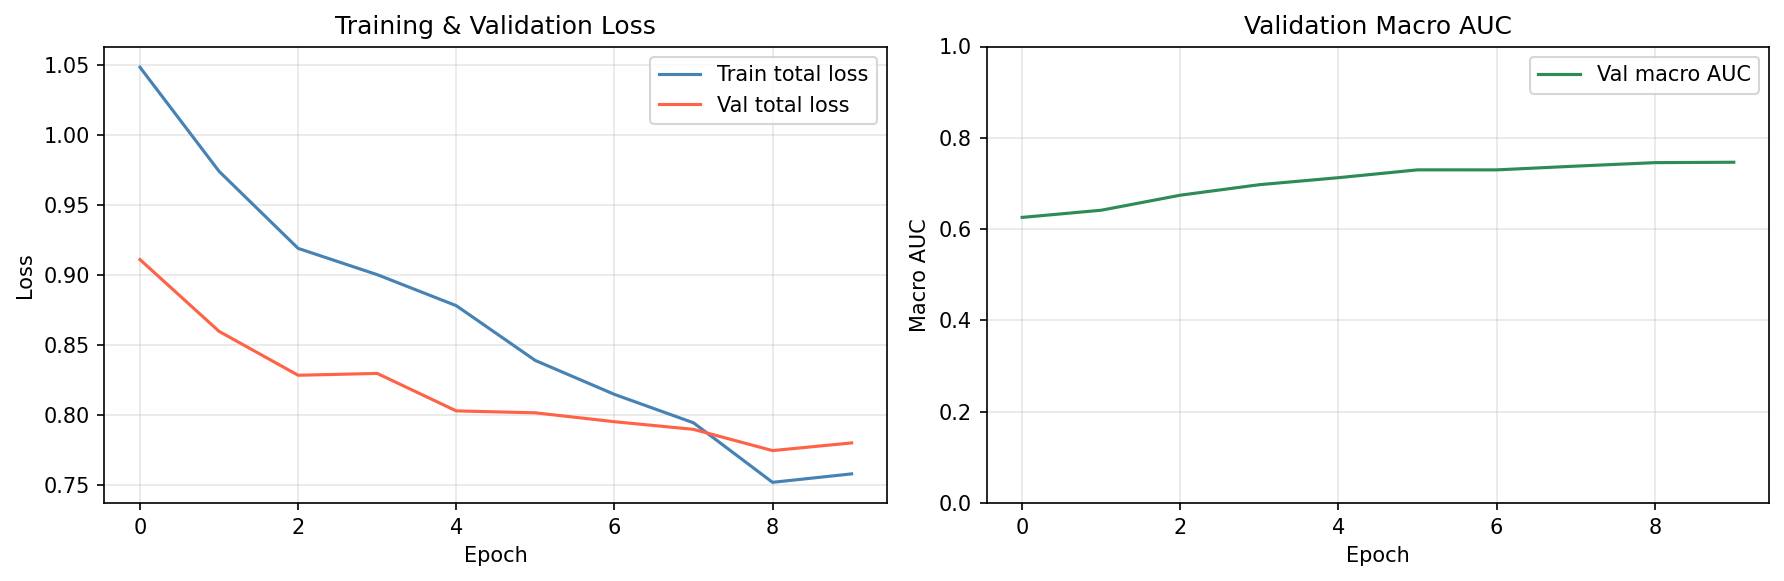
\includegraphics[width=\textwidth]{figures/resnet50_attention_log_curves.png}
    \caption{ResNet50-Attn}
  \end{subfigure}\hfill
  \begin{subfigure}[b]{0.48\textwidth}
    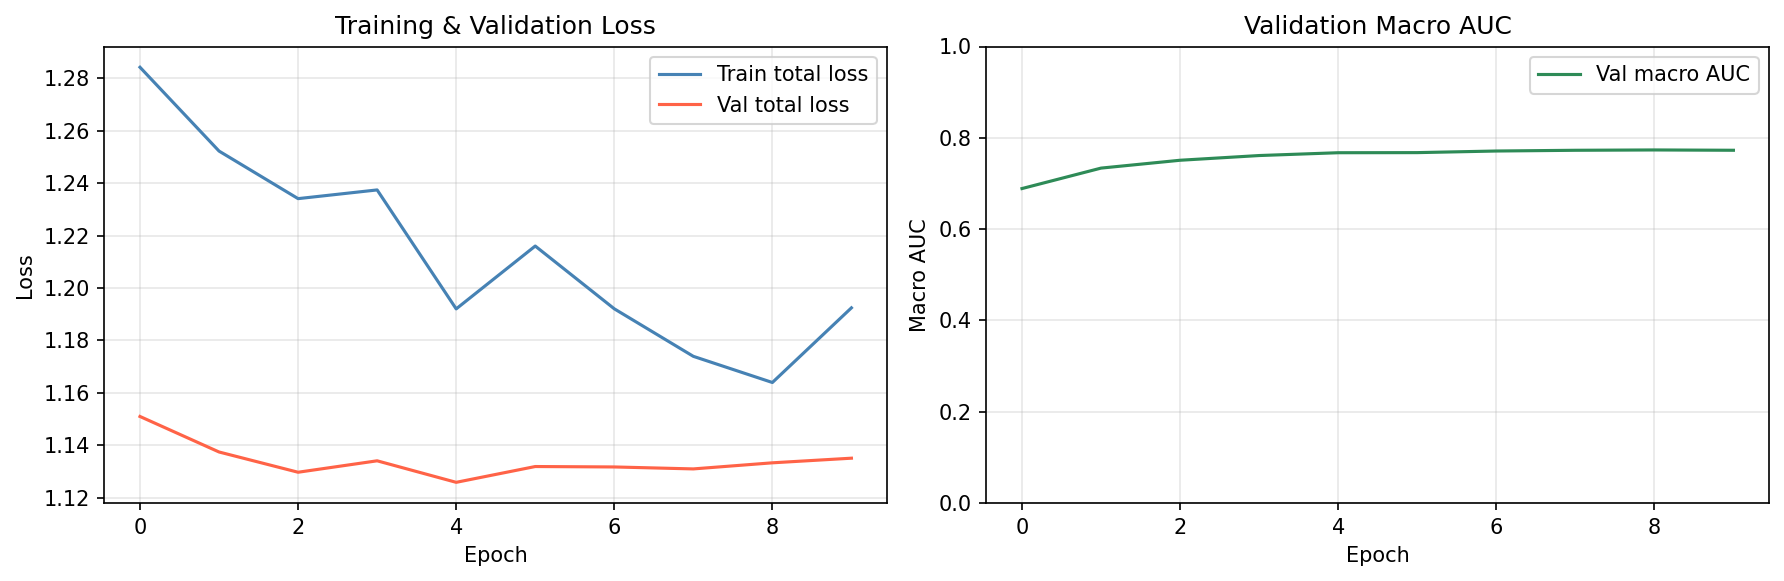
\includegraphics[width=\textwidth]{figures/efficientnet_b0_baseline_log_curves.png}
    \caption{EfficientNet-B0-Base}
  \end{subfigure}

  \medskip
  \begin{subfigure}[b]{0.48\textwidth}
    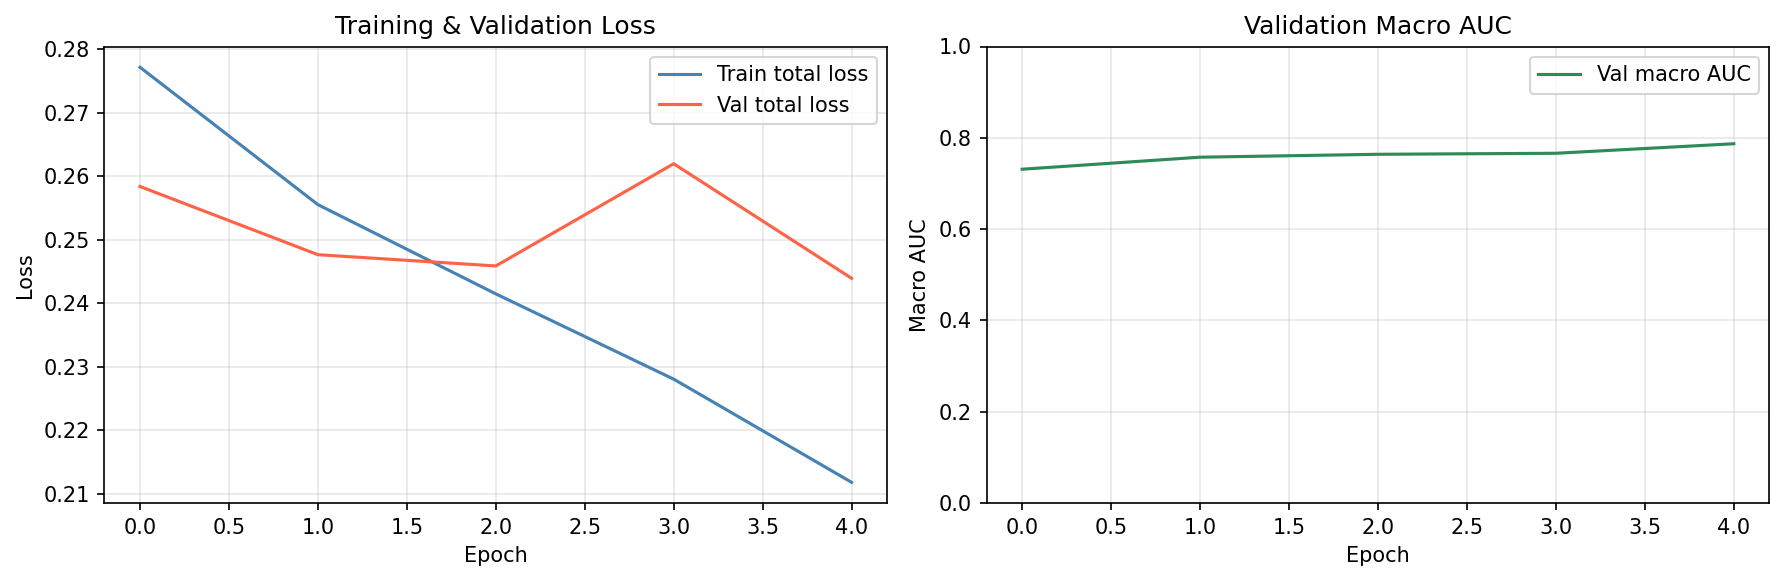
\includegraphics[width=\textwidth]{figures/resnet50_attention_no_lattn_log_curves.png}
    \caption{ResNet50-NoLattn}
  \end{subfigure}\hfill
  \begin{subfigure}[b]{0.48\textwidth}
    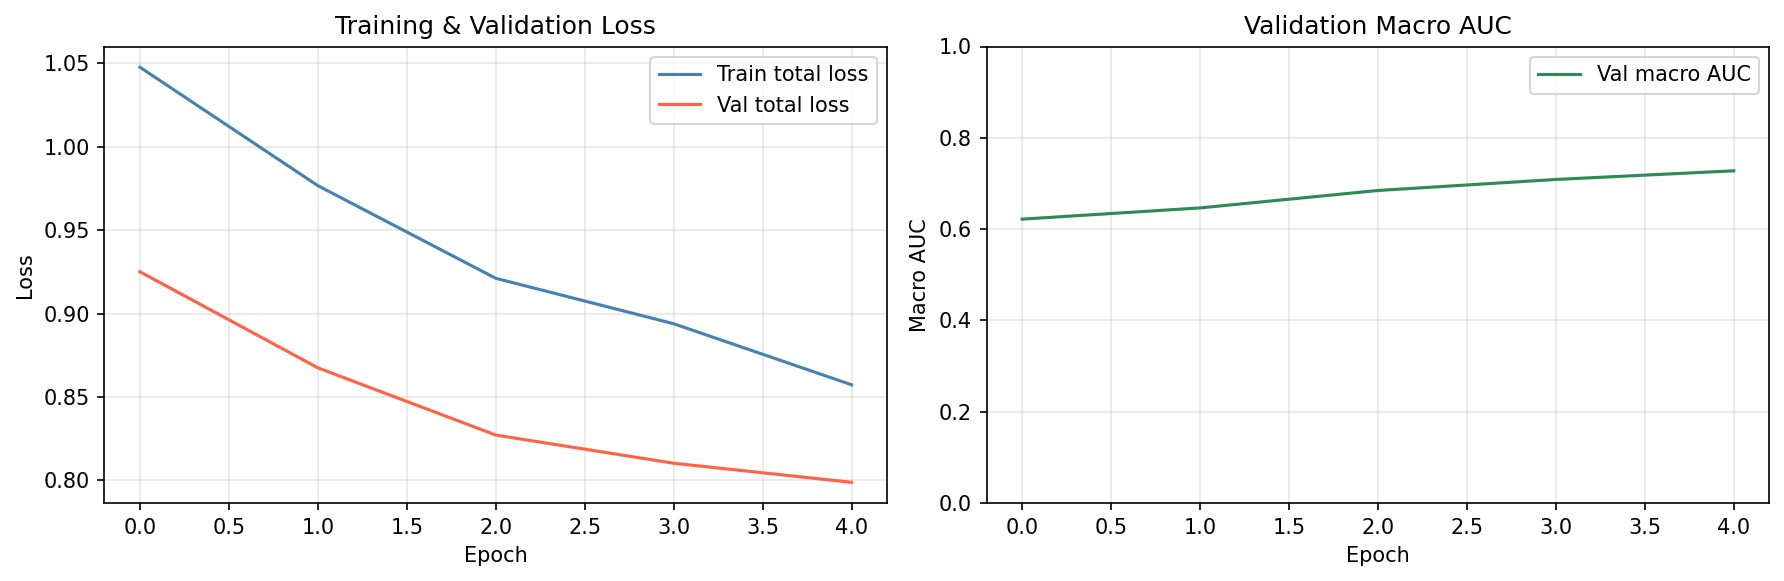
\includegraphics[width=\textwidth]{figures/resnet50_attention_no_lcorr_log_curves.png}
    \caption{ResNet50-NoLcorr}
  \end{subfigure}
  \caption{Training loss and validation AUC curves for six of the seven model
    configurations. Attention variants exhibit slightly more volatile early-epoch
    training due to the additional attention and correlation loss signals.}
  \label{fig:training_curves}
\end{figure}

\begin{figure}[H]
  \centering
  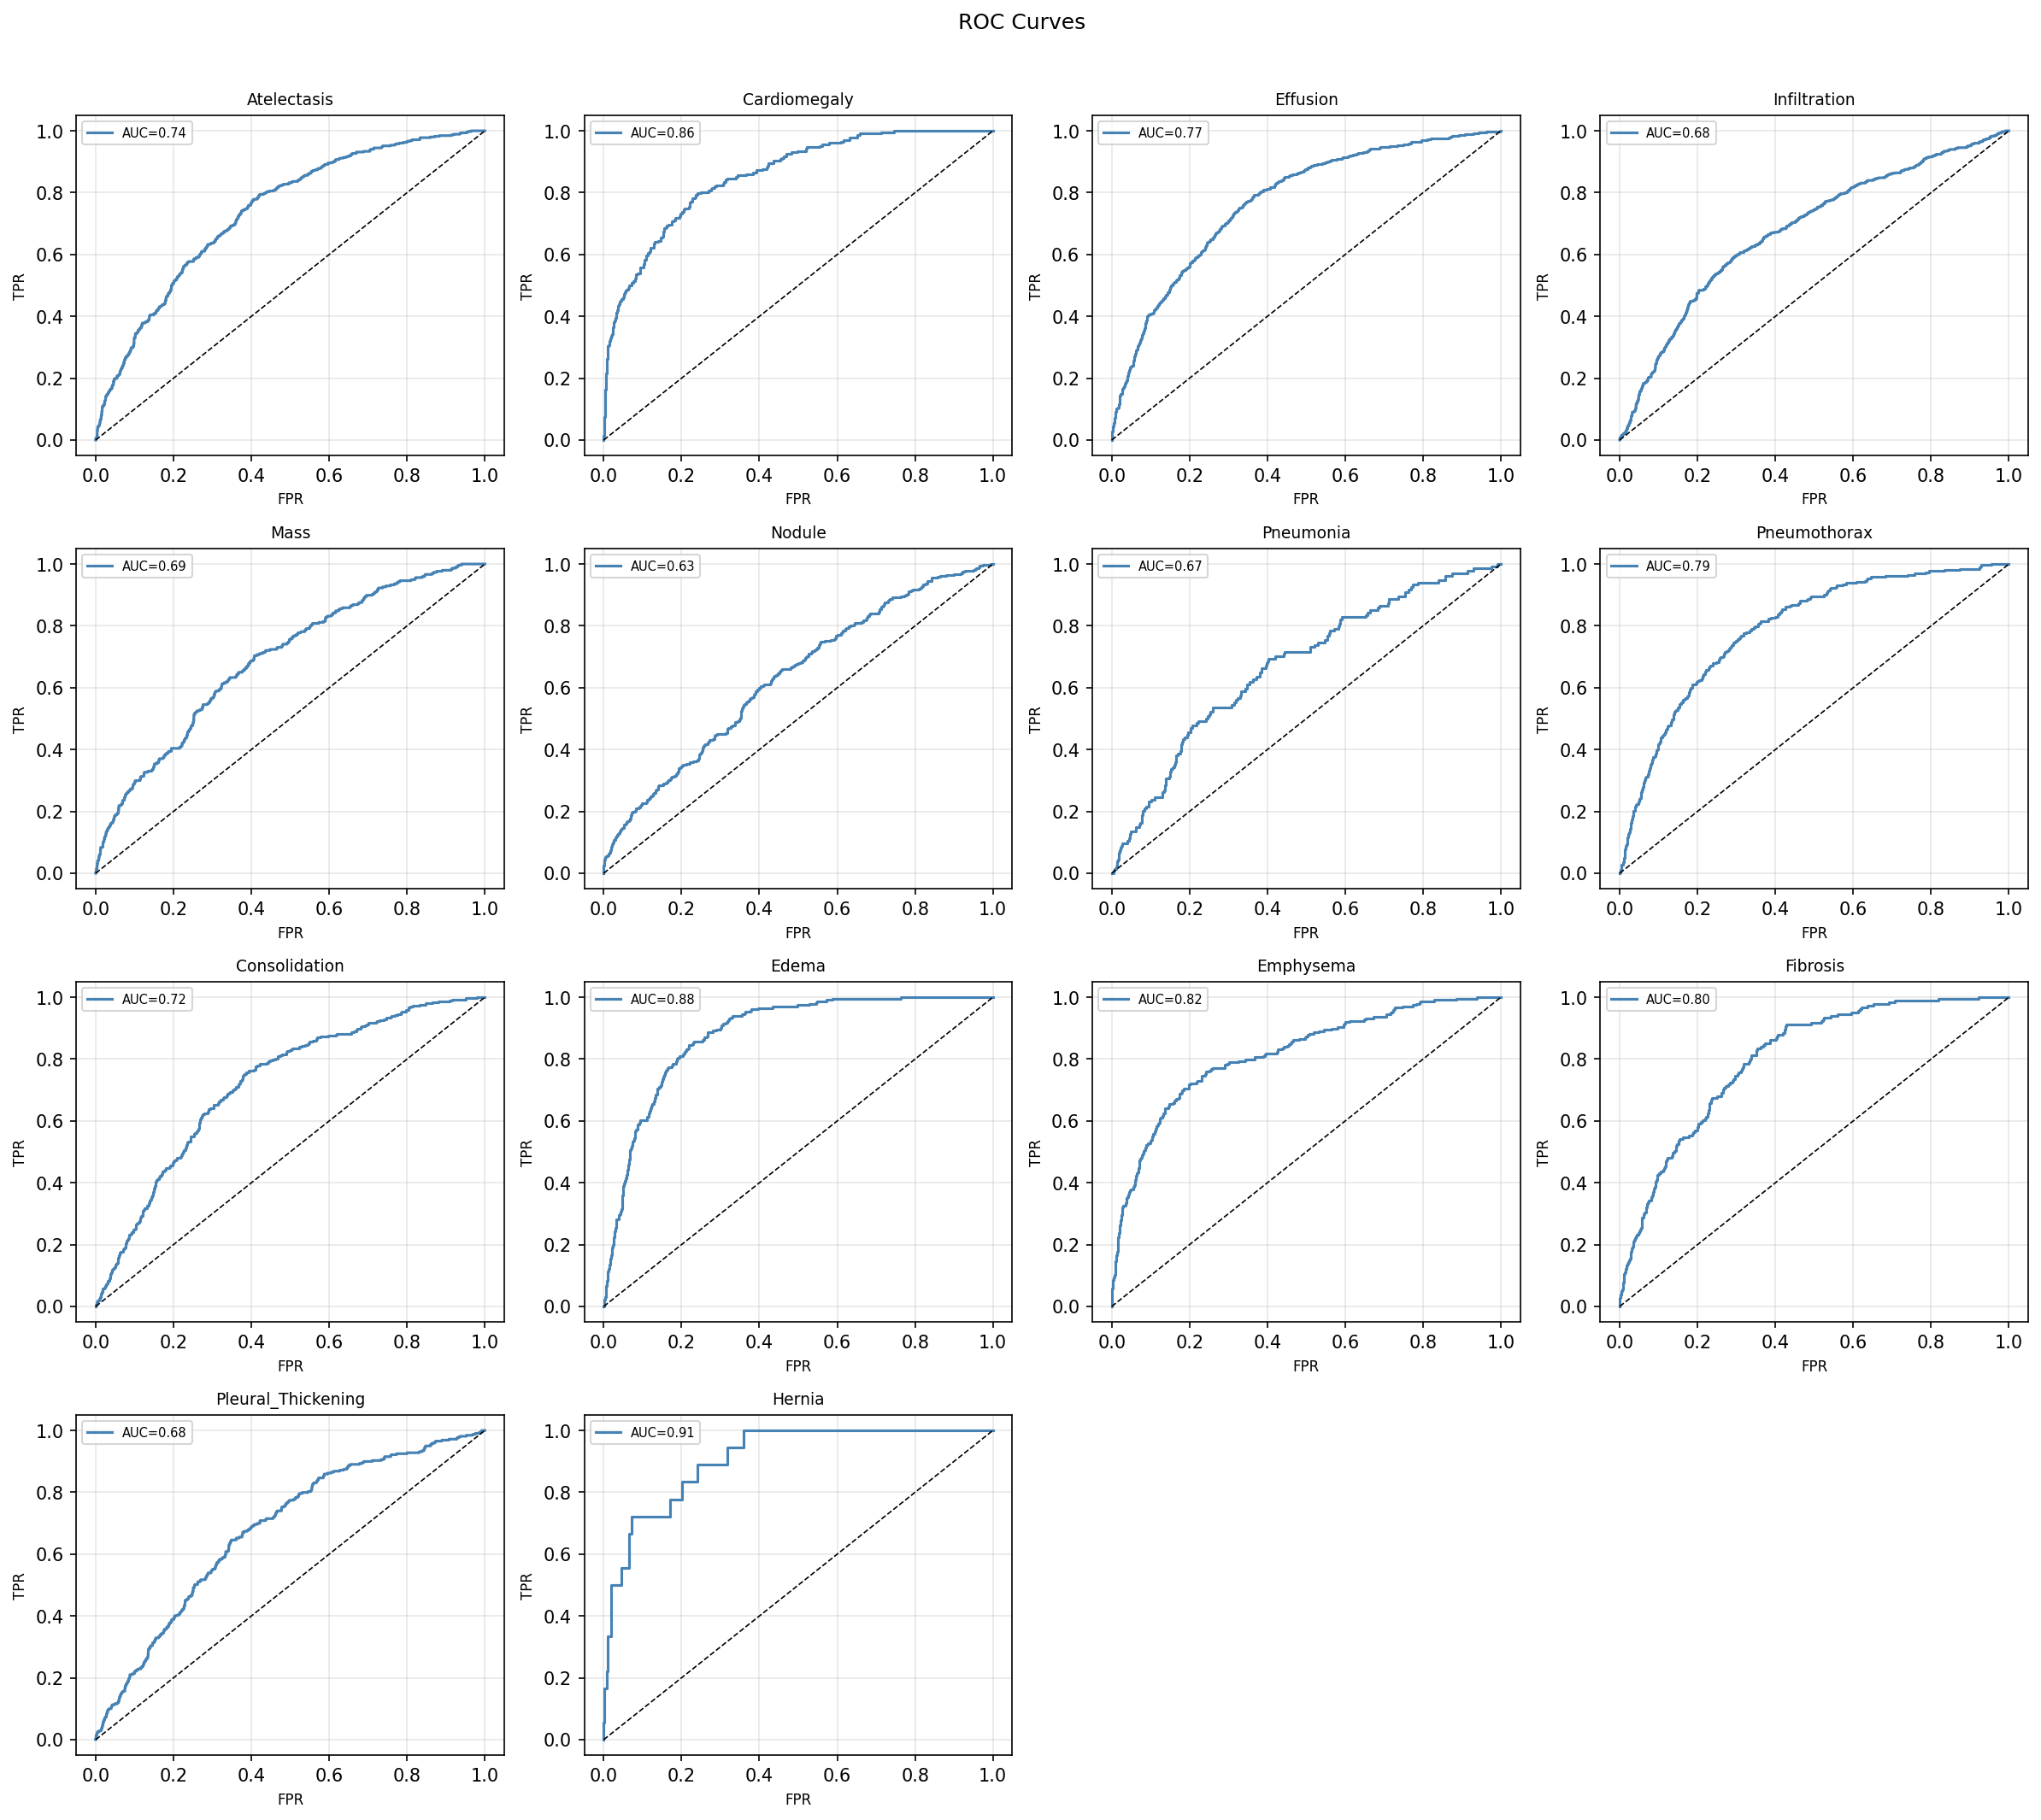
\includegraphics[width=\textwidth]{figures/ROC_Curves_roc.png}
  \caption{Per-class ROC curves for ResNet50-Base (macro AUC~=~0.843), the
    best-performing model. Cardiomegaly, Emphysema, and Hernia achieve the highest
    individual AUC; Infiltration remains the most challenging class (AUC~=~0.692).}
  \label{fig:roc}
\end{figure}

\begin{figure}[H]
  \centering
  \includegraphics[width=0.96\textwidth, height=0.82\textheight, keepaspectratio]%
    {figures/heatmap_overlays.png}
  \caption{\small Qualitative localisation on six NIH ChestX-ray14 test images.
    Col~1: input radiograph.
    Col~2: supervised attention $\mathbf{A}_s$ (ours, blue).
    Col~3: Grad-CAM baseline (red).
    Col~4: clinician ground-truth box (green).
    Supervised attention maps align more closely with annotated disease regions.}
  \label{fig:localization}
\end{figure}

% ─────────────────────────────────────────────────────────────
\section{Discussion}
% ─────────────────────────────────────────────────────────────

\subsection{Classification vs Localisation Trade-off}

The full variant (ResNet50-Attn) achieves a macro AUC of 0.7603 compared to 0.8434 for
ResNet50-Base, a reduction of 0.0831 ($-9.9\%$). DeLong's test confirms this difference
is statistically significant across all 14 disease classes (minimum $p < 3\times10^{-31}$).
This classification cost is the direct price of explanation supervision: forcing the
attention map to align with bounding-box masks introduces a structural constraint that
partially competes with unconstrained classification optimisation. The same pattern holds
for DenseNet121: DenseNet121-Attn achieves 0.7475 vs.\ 0.7911 for DenseNet121-Base
($-0.0436$, minimum DeLong $p < 2\times10^{-17}$). Macro recall is broadly stable across
configurations (0.70--0.82), suggesting the AUC drop is driven by precision-side
trade-offs rather than a collapse in sensitivity. The practical question is whether the
localisation gain justifies this trade-off; Section~\ref{sec:loc_faith} argues it does.

\subsection{Localisation Faithfulness}
\label{sec:loc_faith}

Our supervised attention achieves mean IoU of 0.2991 vs.\ 0.2220 for Grad-CAM on
ResNet50 ($+34.7\%$ relative improvement, $\Delta\text{IoU} = +0.0771$), and
pointing-game accuracy of 0.5063 vs.\ 0.4810 ($+5.3$ pp). This directly answers
\textbf{RQ1}: explanation supervision measurably improves localisation faithfulness
relative to the post-hoc Grad-CAM baseline. For DenseNet121, supervised attention achieves
IoU 0.3178 vs.\ Grad-CAM 0.3120 ($\Delta\text{IoU} = +0.0058$), a smaller but positive
margin. DenseNet121 baselines already achieve higher Grad-CAM IoU (0.3120 vs.\ ResNet50's
0.2220), suggesting the denser feature reuse in DenseNet architectures produces naturally
more spatially coherent activations. The smaller gain for DenseNet121-Attn may therefore
reflect a ceiling effect rather than architectural incompatibility. Notably,
pointing-game accuracy for DenseNet121-Attn (0.4684) is lower than its Grad-CAM baseline
(0.5570), indicating that while attention maps achieve higher overlap area (IoU), the peak
activation point is less reliably centred within the bounding box---possibly because the
class-agnostic union-mask supervision diffuses attention across multiple co-occurring
findings.

\subsection{Ablation Insights}

$\mathcal{L}_{\text{attn}}$ alone accounts for the majority of the localisation gain:
ResNet50-NoLcorr ($+\mathcal{L}_{\text{attn}}$ only) achieves IoU~=~0.3096 vs.\
baseline 0.2220 ($+39.5\%$ relative), and pointing-game~=~0.4684. Adding
$\mathcal{L}_{\text{corr}}$ (full ResNet50-Attn) yields IoU~=~0.2991 and
pointing-game~=~0.5063---slightly lower IoU but higher pointing-game accuracy,
suggesting $\mathcal{L}_{\text{corr}}$ redistributes attention to better centre on
disease foci. $\mathcal{L}_{\text{corr}}$ alone (ResNet50-NoLattn) provides no
localisation benefit: IoU~=~0.1469, pointing-game~=~0.2911, both well below baseline.
This is expected---$\mathcal{L}_{\text{corr}}$ is a label-space regulariser with no
direct spatial supervision signal. Its value is classification-side: ResNet50-NoLattn
achieves macro AUC~=~0.8000, the highest among all ResNet50 variants, just 0.043 below
the unconstrained baseline. This confirms \textbf{RQ2}: $\mathcal{L}_{\text{attn}}$ is
the primary driver of localisation gain, while $\mathcal{L}_{\text{corr}}$ partially
recovers classification AUC without contributing to spatial faithfulness. The full model
($+\mathcal{L}_{\text{attn}}+\mathcal{L}_{\text{corr}}$, AUC~=~0.7603,
IoU~=~0.2991, PG~=~0.5063) represents the best overall trade-off among ResNet50
configurations.

\subsection{Backbone Comparison}

ResNet50-Base achieves the best baseline macro AUC (0.8434), outperforming both
DenseNet121-Base (0.7911) and EfficientNet-B0-Base (0.7920). The near-identical
performance of DenseNet121 and EfficientNet-B0 baselines suggests the classification task
is not strongly backbone-sensitive at this dataset scale, and that the class-balanced
training subset may limit the advantage of more expressive architectures. Hernia is the
most discriminable class across all models (ResNet50-Base AUC~=~1.000), likely due to its
visually distinctive appearance. Infiltration is consistently the hardest class
(0.679--0.692), consistent with its high visual similarity to normal lung texture.
ResNet50's stronger baseline AUC likely reflects its simpler spatial feature hierarchy
being better suited to fine-grained binary grid mask supervision. DenseNet121's feature
reuse may diffuse spatial gradients, making attention supervision less sharp. This
partially answers \textbf{RQ3}: backbone choice interacts with attention supervision,
with ResNet50 offering the best classification baseline and DenseNet121 achieving
competitive localisation IoU despite lower classification AUC.

\subsection{Limitations}

Several limitations should be acknowledged. First, $\mathbf{A}_s$ is a class-agnostic
map supervised against the union of all bounding boxes in an image, meaning in
multi-finding images the attention must compromise among spatially distinct regions.
Second, bounding-box annotations cover only $\approx$0.8\% of ChestX-ray14 images, so
the majority of training examples contribute only via the sparsity regulariser. Third,
computational constraints required a $\approx$5,000-image training subset; full-dataset
experiments may alter results. Fourth, evaluation is restricted to the 8 findings with
bounding-box annotations; the remaining 6 are assessed only on classification metrics.

% ─────────────────────────────────────────────────────────────
\section{Conclusion}
% ─────────────────────────────────────────────────────────────

We presented an explanation-supervised attention CNN for multi-label thoracic disease
classification on NIH ChestX-ray14. By promoting the spatial attention map from an
implicit intermediate computation to a first-class trainable output supervised by
clinician-annotated bounding boxes, we demonstrated that the faithfulness of spatial
explanations can be improved as part of training---without incurring additional inference
cost compared to standard CNN classifiers.

The composite attention loss (Dice + MSE on annotated images; L1 sparsity on unannotated
images) and the label-correlation regulariser together constitute a principled extension
of the standard multi-label classification objective. Ablations isolate the contribution
of each component, and DeLong's test provides statistical grounding for AUC comparisons.

This work contributes a new perspective on CNN interpretability for medical imaging:
\emph{explanations should be part of training, not an afterthought.} The approach is
applicable wherever weak localisation labels (bounding boxes, click annotations, or coarse
segmentations) are available alongside classification labels.

\subsection{Future Work}

Natural extensions include: (1)~per-class attention maps, where each finding has its own
spatial module trained against finding-specific bounding boxes; (2)~extension to larger
annotated CXR corpora (CheXpert, PadChest); (3)~curriculum supervision that progressively
increases $\lambda_1$ as training stabilises; (4)~adaptation to transformer architectures
(e.g., supervising ViT attention heads); and (5)~a clinical pilot study assessing whether
the more faithful heat maps improve radiologist trust and efficiency.

% ─────────────────────────────────────────────────────────────
\bibliographystyle{abbrvnat}
\bibliography{references}
% ─────────────────────────────────────────────────────────────

% ─────────────────────────────────────────────────────────────
\appendix
\section{Full Per-Class ROC-AUC}
\label{app:perclass}
% ─────────────────────────────────────────────────────────────

\begin{table}[H]
  \centering
  \caption{Full per-class ROC-AUC for all 14 thoracic findings across the five main
           model configurations. Best value in each row is \textbf{bold}.}
  \label{tab:perclass}
  \begin{tabular}{lccccc}
    \toprule
    \textbf{Finding} & \textbf{R50-Base} & \textbf{DN121-Base} &
      \textbf{EffNet-Base} & \textbf{R50-Attn} & \textbf{DN121-Attn} \\
    \midrule
    Atelectasis        & \textbf{0.795} & 0.764 & 0.762 & 0.738 & 0.705 \\
    Cardiomegaly       & \textbf{0.945} & 0.904 & 0.897 & 0.856 & 0.850 \\
    Effusion           & \textbf{0.818} & 0.799 & 0.793 & 0.773 & 0.741 \\
    Infiltration       & \textbf{0.692} & 0.675 & 0.680 & 0.679 & 0.661 \\
    Mass               & \textbf{0.858} & 0.773 & 0.760 & 0.690 & 0.698 \\
    Nodule             & \textbf{0.725} & 0.698 & 0.689 & 0.633 & 0.632 \\
    Pneumonia          & \textbf{0.796} & 0.681 & 0.693 & 0.672 & 0.646 \\
    Pneumothorax       & \textbf{0.871} & 0.834 & 0.832 & 0.792 & 0.748 \\
    Consolidation      & \textbf{0.763} & 0.725 & 0.712 & 0.720 & 0.705 \\
    Edema              & \textbf{0.926} & 0.889 & 0.892 & 0.882 & 0.872 \\
    Emphysema          & \textbf{0.947} & 0.905 & 0.888 & 0.817 & 0.786 \\
    Fibrosis           & \textbf{0.851} & 0.823 & 0.824 & 0.803 & 0.789 \\
    Pleural\_Thickening & \textbf{0.821} & 0.760 & 0.723 & 0.679 & 0.690 \\
    Hernia             & \textbf{1.000} & 0.847 & 0.942 & 0.910 & 0.941 \\
    \midrule
    \textbf{Macro Avg} & \textbf{0.843} & 0.791 & 0.792 & 0.760 & 0.748 \\
    \bottomrule
  \end{tabular}
\end{table}

\end{document}
